\section{Map Node Locking}
\label{prototype:MapNodeLocking}
With my previous iterations, every time the map was loaded the nodes would have a different location. 
Whilst this ensured graphs were optimally laid out, it did result in difficulty finding nodes as muscle memory couldn't be built.

To improve this I have added the feature to 'lock' nodes into a position. Anytime a node is manually dragged around the canvas it becomes locked. Locked nodes then 'remember' their position any time they are redrawn on the graph. All nodes can be 'unlocked' by the top button (when pressed the nodes will automatically reorder themselves most optimally) 

Nodes that are locked are shown with a purple border colour , this is to ensure the user can easily identify which nodes are locked and which are not

\begin{figure}[H]
    \centering
    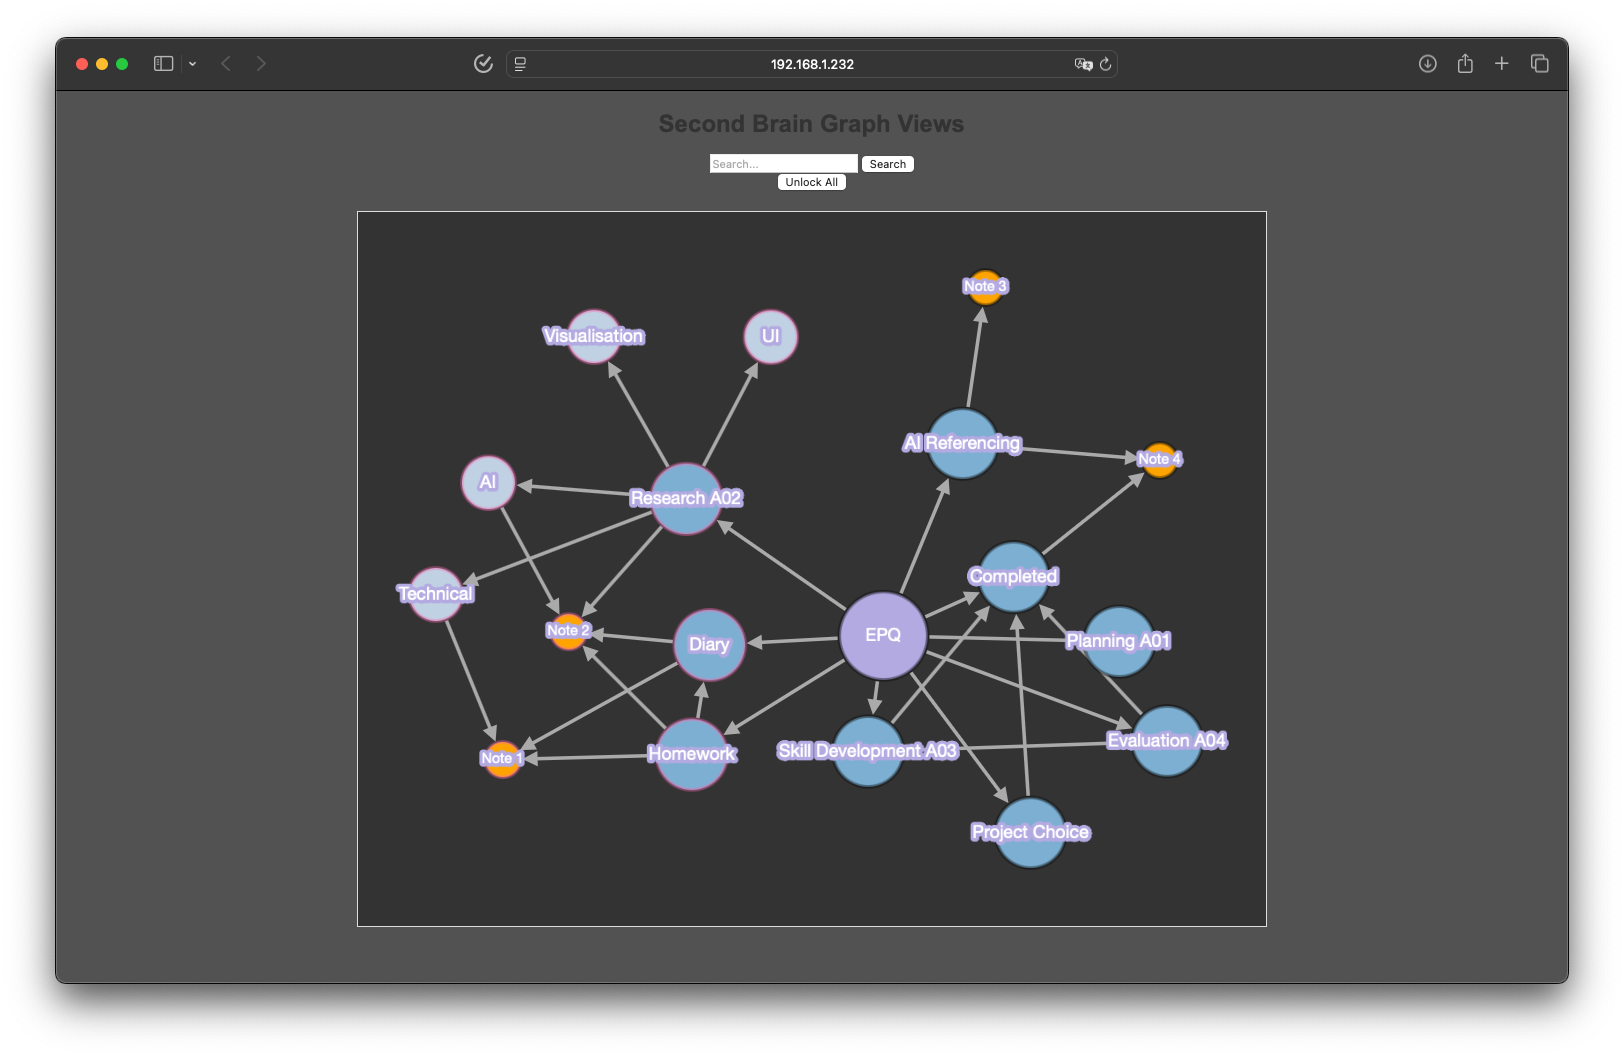
\includegraphics[width=0.8\textwidth]{Prototype/8_MapNodeLocking/media/prototype.png}
    \caption{Map Node Locking Prototype}
\end{figure}
